\chapter{Electrónica}

\section{Diagrama en bloque de las partes}

   \begin{figure}[H]
    \centering
    \begin{tikzpicture}[
        node distance=1.8cm, font=\small,
        sensor/.style={rectangle, draw, fill=cyan!30, rounded corners, minimum height=2em, text centered, minimum width=3.5cm},
        mcu/.style={rectangle, draw, fill=green!30, rounded corners, minimum height=2em, text centered, minimum width=3.5cm},
        output/.style={rectangle, draw, fill=blue!30, rounded corners, minimum height=2em, text centered, minimum width=3.5cm},
        power/.style={rectangle, draw, fill=green!30, rounded corners, minimum height=2em, text centered, minimum width=3.5cm},
        interface/.style={rectangle, draw, fill=cyan!30, rounded corners, minimum height=2em, text centered, minimum width=3.5cm},
        arrow/.style={-{Latex[length=3mm, width=2mm]}, thick}
    ]
    
    % Nodos
    \node (power) [power] {Alimentación 5V};
    \node (lpc845) [mcu, below of=power] {MCU (LPC845)};
    \node (max6675) [sensor, left of=lpc845, xshift=-4cm] {MAX6675 (Temperatura tipo K)};
    \node (max31865) [sensor, above of=max6675] {MAX31865 (RTD PT100/PT1000)};
    \node (rpm) [sensor, below of=max6675] {Circuito comparador de RPM};
    \node (presion) [sensor, right of=lpc845, xshift=4cm] {Circuito de presión de aceite};
    \node (oxigeno) [sensor, above of=presion] {Circuito de oxígeno};
    \node (interface) [interface, below of=presion, yshift=-2cm] {Interfaz Digital};
    \node (reles) [output, below of=lpc845, yshift=-2cm] {Circuito de relés (Alarmas)};
    
    % Flechas de conexión
    \draw [arrow] (power) -- (lpc845);
    \draw [arrow] (max6675) -- (lpc845);
    \draw [arrow] (max31865) -- (lpc845);
    \draw [arrow] (rpm) -- (lpc845);
    \draw [arrow] (presion) -- (lpc845);
    \draw [arrow] (oxigeno) -- (lpc845);
    \draw [arrow] (lpc845) -- (reles);
    \draw [arrow] (lpc845) -- (interface);

    \end{tikzpicture}
    \caption{Diagrama en bloques del sistema de monitoreo basado en LPC845, incluyendo la interfaz digital.}
    \label{fig:diagrama_bloques_lpc845_interfaz}
\end{figure}

\section{Sensores utilizados}

\begin{itemize}
    \item \textbf{Termocuplas tipo K:}  
    Sensor de temperatura fabricado con dos metales distintos unidos en un punto de medición.  
    \begin{itemize}
        \item Rango de temperatura: -200 °C a 1,260 °C.  
        \item Alta durabilidad y capacidad de trabajar en entornos extremos.  
        \item Genera un voltaje proporcional a la temperatura.  
    \end{itemize}

    \item \textbf{Termistores PT100 RTD:}  
    Sensor de temperatura basado en resistencia de platino.  
    \begin{itemize}
        \item Alta precisión en un rango de -200 °C a 850 °C.  
        \item Resistencia nominal de 100 ohmios a 0 °C.  
        \item Amplia estabilidad y repetibilidad en mediciones.  
    \end{itemize}

    \item \textbf{Sonda Lambda:}  
    Sensor utilizado para medir la proporción aire-combustible en motores de combustión interna.  
    \begin{itemize}
        \item Proporciona información sobre la combustión eficiente del motor.  
        \item Trabaja típicamente con una señal de voltaje generada por una celda electroquímica.  
        \item Sensible a la cantidad de oxígeno en los gases de escape.  
    \end{itemize}

    \item \textbf{Sensor de presión de aceite (Rotax 912 ULS):}  
    Dispositivo que mide la presión del aceite para garantizar el correcto funcionamiento del motor.  
    \begin{itemize}
        \item Rango de medición típico: 0 a 10 bar.  
        \item Sensores basados en tecnología piezorresistiva.  
        \item Compatible con sistemas de monitoreo del motor Rotax 912 ULS.  
    \end{itemize}

    \item \textbf{Sensor de RPM (Rotax 912 ULS):}  
    Sensor utilizado para medir la velocidad de rotación del motor.  
    \begin{itemize}
        \item Se basa en señales generadas por impulsos del cigüeñal.  
        \item Rango típico de operación del motor: 0 a 5,800 RPM.  
        \item Proporciona datos críticos para el control y monitoreo del rendimiento.  
    \end{itemize}
\end{itemize}

     
    
\section{Software usado para el desarrollo de esquemáticos y PCB}

% Inclusión del logo de Proteus 8
\begin{figure}[h]
    \centering
    
\includegraphics[width=0.3\textwidth]{Imagenes/logo proteus (2).png}
    \caption{Proteus 8}
    \label{fig:logo_proteus}
\end{figure}

Para el diseño y simulación de los circuitos en este proyecto, se utilizó el software **Proteus 8**, conocido por su robustez y versatilidad en el desarrollo de sistemas electrónicos. En particular, se aprovecharon las herramientas de simulación, diseño esquemático y diseño de PCB que ofrece este software.

Entre las características destacadas de Proteus 8 utilizadas en este proyecto, se encuentran:

\begin{itemize}
    \item Simulación: % Descripción de la simulación
    Permite realizar simulaciones avanzadas de circuitos electrónicos, incluyendo microcontroladores, componentes analógicos y digitales. Esto posibilita validar el comportamiento del circuito antes de fabricarlo.
    \item Diseño esquemático: % Descripción del diseño esquemático
    Ofrece una interfaz intuitiva para crear esquemáticos detallados, con una amplia librería de componentes que facilita el desarrollo y la documentación del diseño.
    \item Diseño de PCB: % Descripción del diseño de PCB
    Proporciona herramientas para el diseño de PCB, permitiendo tanto el ruteo automático como manual. Además, incluye verificación de reglas de diseño (DRC), lo que asegura la correcta fabricación de la placa.
\end{itemize}

El uso combinado de estas funcionalidades permitió desarrollar y validar el circuito de manera integral, reduciendo posibles errores y optimizando el proceso de diseño

\section{Esquemático de cada bloque}

En esta sección se presentan los distintos esquemáticos correspondientes a cada bloque del proyecto. A continuación se listan:

\subsection{Amplificador AD620 (Sonda Lambda)}
\begin{figure}[H]
    \centering
    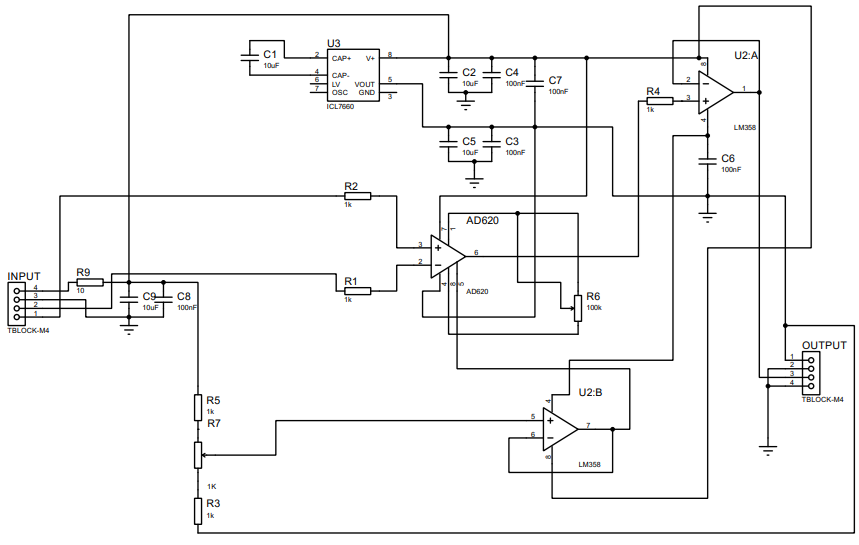
\includegraphics[width=0.8\textwidth]{Imagenes/AD620.png}
    \caption{Esquemático del Amplificador AD620 (SONDA LAMBDA}
    \label{fig:ad620}
\end{figure}
\textbf{Descripción:} Este bloque muestra el circuito del amplificador instrumental AD620 utilizado para amplificar señales pequeñas provenientes de la Sonda Lambda

\subsection{Acondicionador de señal para RPM: Comparador LM311}
\begin{figure}[H]
    \centering
    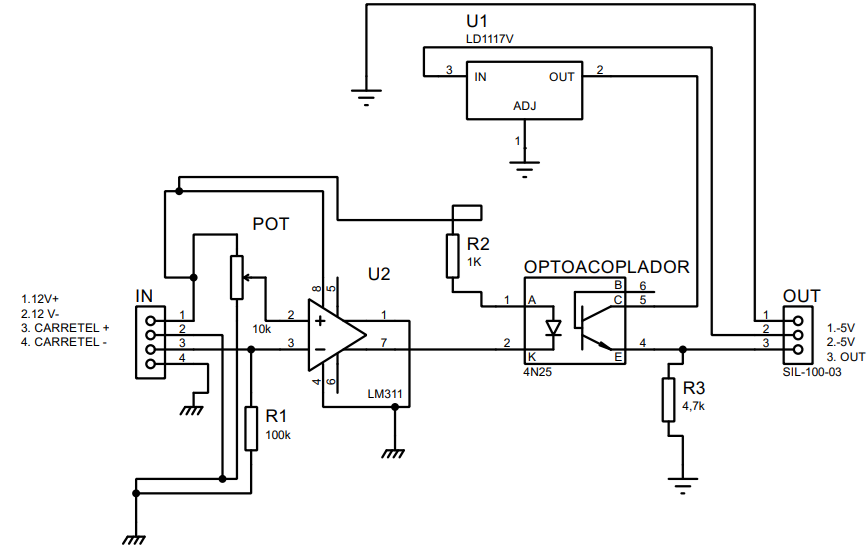
\includegraphics[width=0.8\textwidth]{Imagenes/Comparador de RPM.png}
    \caption{Esquemático del Comparador LM311 para RPM}
    \label{fig:lm311}
\end{figure}
\textbf{Descripción:} Este circuito acondiciona la señal de RPM utilizando el comparador LM311 para generar una señal digital adecuada.

\subsection{Divisor de voltaje para el sensor de presión de aceite}
\begin{figure}[H]
    \centering
    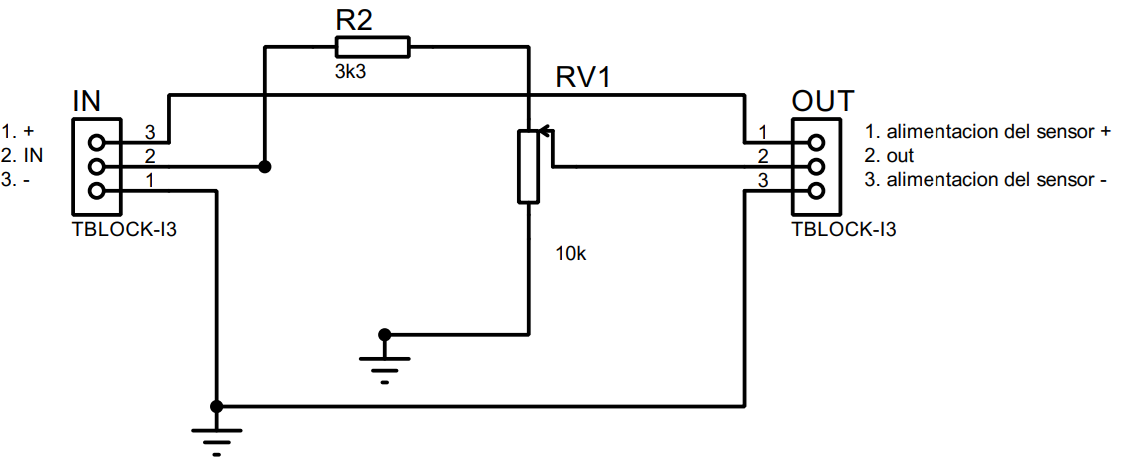
\includegraphics[width=0.8\textwidth]{Imagenes/Divisor de voltaje para presion de aceite.png}
    \caption{Esquemático del divisor de voltaje para el sensor de presión de aceite}
    \label{fig:divisor_presion}
\end{figure}
\textbf{Descripción:} El divisor de voltaje se utiliza para ajustar la señal de salida del sensor de presión de aceite para su correcta lectura por el microcontrolador.

\subsection{Placa general de conexiones: Rev-Control}
\begin{figure}[H]
    \centering
    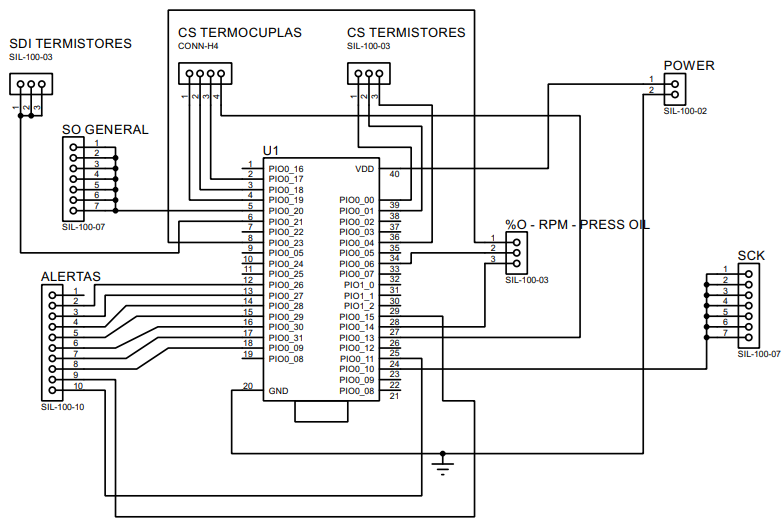
\includegraphics[width=0.8\textwidth]{Imagenes/Placa rev control.png}
    \caption{Esquemático general del Rev-Control}
    \label{fig:rev_control}
\end{figure}
\textbf{Descripción:} Este esquemático muestra la placa general de conexiones, incluyendo la integración de todos los módulos previamente mencionados.

\subsection{Sistema de Alarmas con Relés}
\begin{figure}[H]
    \centering
    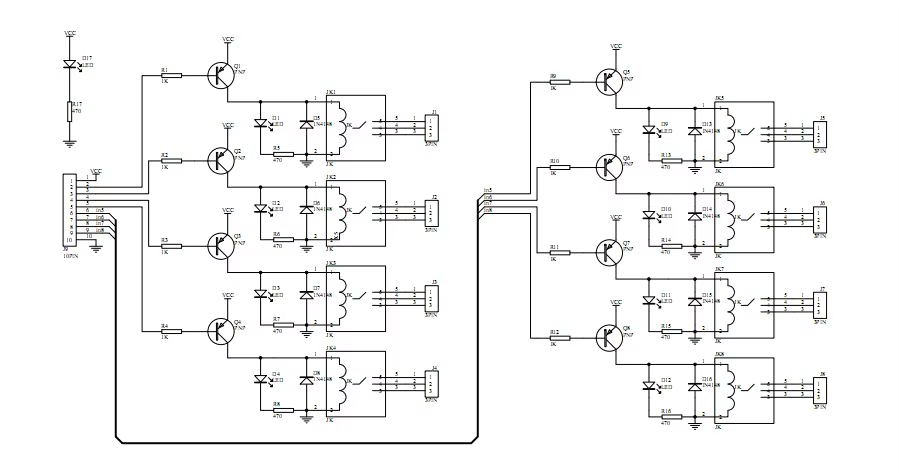
\includegraphics[width=0.8\textwidth]{Imagenes/Placa reles 8 canales.png}
    \caption{Esquemático del Sistema de Alarmas con Relés}
    \label{fig:alarmas_reles}
\end{figure}
\textbf{Descripción:} El sistema de alarmas utiliza relés para activar diferentes señales visuales y auditivas ante eventos críticos.

\subsection{MAX6675 para Termocupla}
\begin{figure}[H]
    \centering
    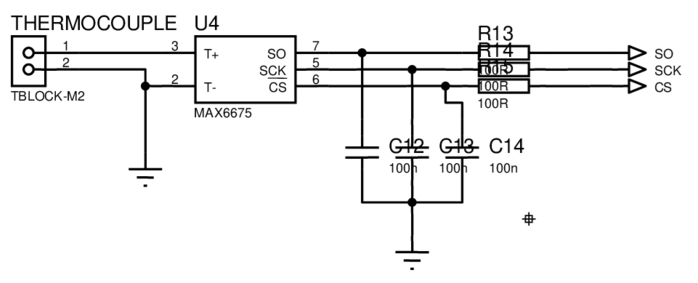
\includegraphics[width=0.8\textwidth]{Imagenes/MAX6675.png}
    \caption{Esquemático del MAX6675 para Termocupla}
    \label{fig:max6675}
\end{figure}
\textbf{Descripción:} El módulo MAX6675 se utiliza para la lectura de temperaturas a través de una termocupla tipo K, proporcionando una señal digital al microcontrolador.

\subsection{MAX31865 para Termistor}
\begin{figure}[H]
    \centering
    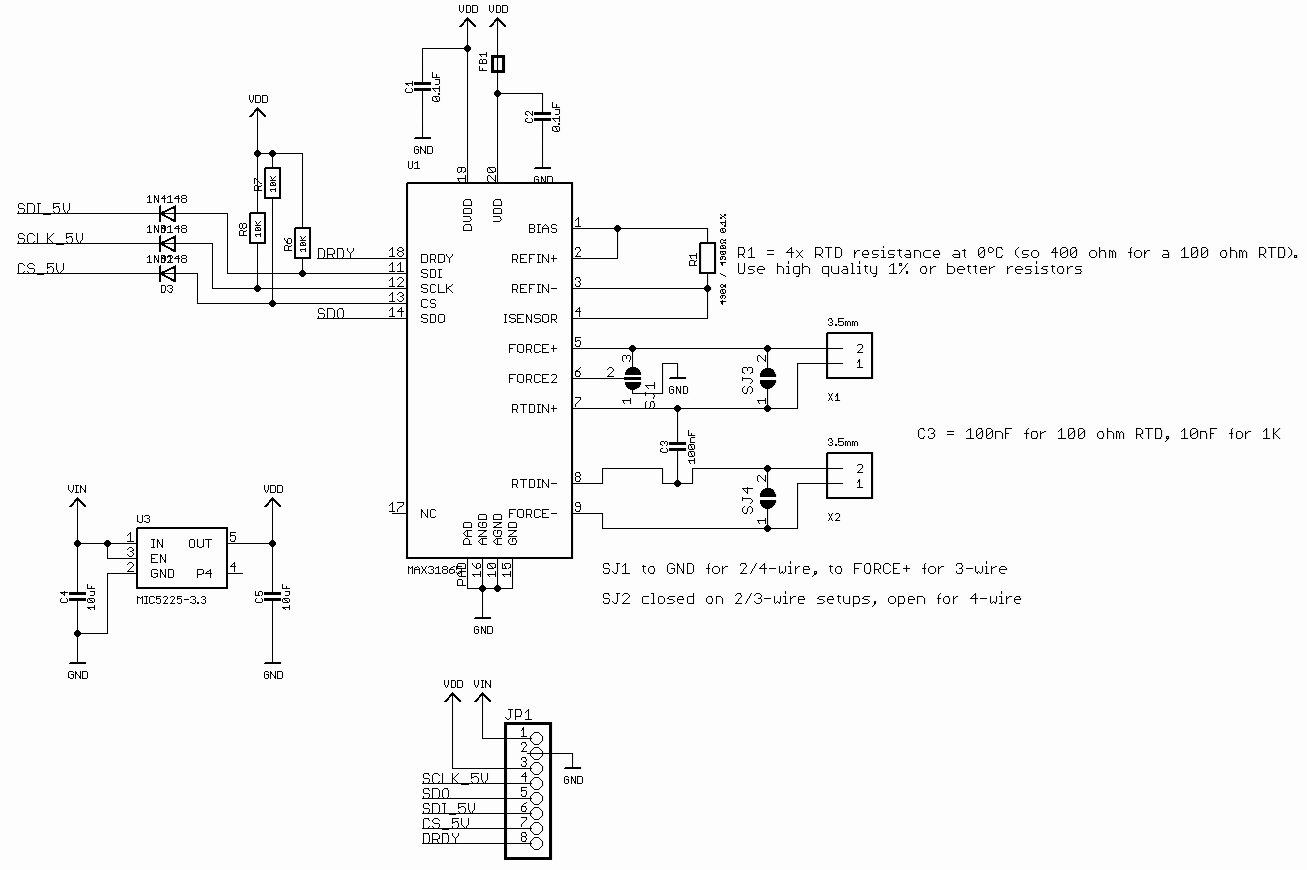
\includegraphics[width=0.8\textwidth]{Imagenes/MAX31865.png}
    \caption{Esquemático del MAX31865 para Termistor}
    \label{fig:max31865}
\end{figure}
\textbf{Descripción:} El módulo MAX31865 se utiliza para la lectura de termistores PT100/PT1000, permitiendo una medición precisa de la temperatura.

\newpage
\section{PCB de cada bloque}
Aquí se muestran los diseños de PCB correspondientes a cada bloque del sistema.

\begin{tabular}{ccc} % Establece 3 columnas
  \multicolumn{1}{c}{} & \multicolumn{1}{c}{} & \multicolumn{1}{c}{} \\ % Fila vacía para separación
  % Primera fila: tres columnas
  \begin{minipage}{0.32\textwidth}
    \centering
    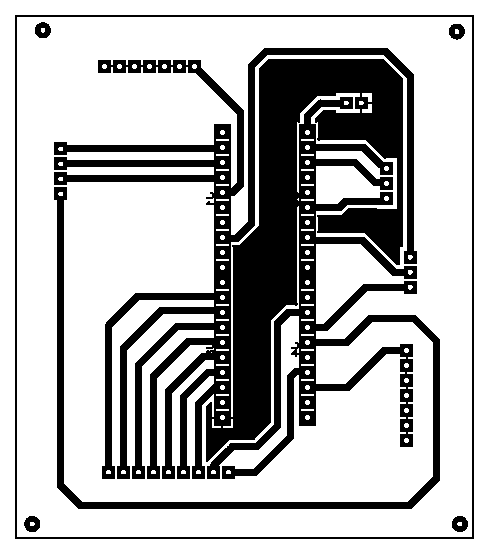
\includegraphics[width=\textwidth,height=0.2\textheight,keepaspectratio]{PCBS/LPC PCB.pdf} % Inserta el primer PDF como imagen
  \end{minipage} &
  \begin{minipage}{0.32\textwidth}
    \centering
    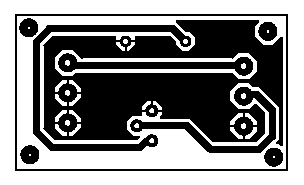
\includegraphics[width=\textwidth,height=0.2\textheight,keepaspectratio]{PCBS/Divisor de voltaje PCB.pdf} % Inserta el segundo PDF como imagen
  \end{minipage} &
  \begin{minipage}{0.32\textwidth}
    \centering
    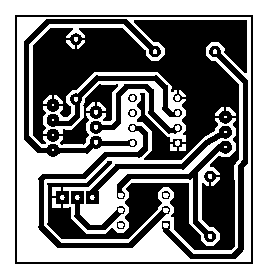
\includegraphics[width=\textwidth,height=0.2\textheight,keepaspectratio]{PCBS/Comparador PCB.pdf} % Inserta el tercer PDF como imagen
  \end{minipage} \\
  
  \vspace{1em} % Espacio entre las filas
  
  % Segunda fila: tres columnas
  \begin{minipage}{0.32\textwidth}
    \centering
    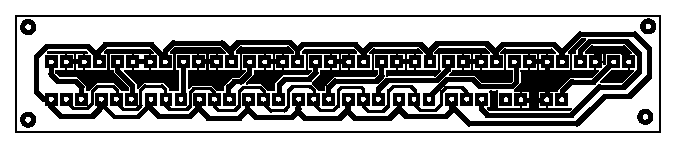
\includegraphics[width=\textwidth,height=0.2\textheight,keepaspectratio]{PCBS/Alarmas.pdf} % Inserta el cuarto PDF como imagen
  \end{minipage} &
  \begin{minipage}{0.32\textwidth}
    \centering
    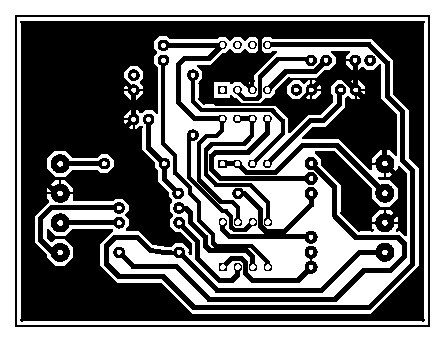
\includegraphics[width=\textwidth,height=0.2\textheight,keepaspectratio]{PCBS/AD620 PCB.pdf} % Inserta el quinto PDF como imagen
  \end{minipage} &
  \begin{minipage}{0.32\textwidth}
    \centering
    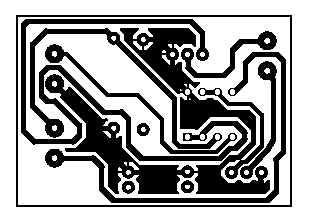
\includegraphics[width=\textwidth,height=0.2\textheight,keepaspectratio]{PCBS/Acondicionador PCB.pdf} % Inserta el sexto PDF como imagen
  \end{minipage} \\
\end{tabular}


\section{Especificaciones de Alimentación y Potencia}

Todos los circuitos están alimentados por una batería de 12V 7Ah de plomo-ácido gel. A continuación, se detallan las especificaciones de alimentación y consumo de cada módulo, incluyendo el LPC845:

\begin{table}[h!]
\centering
\resizebox{\textwidth}{!}{%
\begin{tabular}{|l|c|c|c|}
\hline
\textbf{Módulo} & \textbf{Voltaje de Alimentación (V)} & \textbf{Consumo (mA)} & \textbf{Potencia (W)} \\ \hline
Circuito Comparador (LM311 + Optoacoplador) & 12 & 15 & 0.18 \\ \hline
Divisor de Voltaje & 12 & 10 & 0.12 \\ \hline
Amplificador AD620 & $\pm$ 12 (Regulado) & 30 & 0.72 \\ \hline
Módulo de Relés Optoacoplados & 12 & 300 (8 relés activos) & 3.60 \\ \hline
MAX6675 & 3.3 (Regulado) & 5 & 0.0165 \\ \hline
MAX31865 & 3.3 (Regulado) & 3 & 0.0099 \\ \hline
Monitor Kinseal AMZ070W01RAGD & 12 & 400 & 4.80 \\ \hline
LPC845 & 5 (Regulado) & 50 & 0.165 \\ \hline
\textbf{Total} & - & \textbf{803} & \textbf{9.98} \\ \hline
\end{tabular}%
}
\caption{Consumo de energía de los circuitos alimentados por la batería de 12V 7Ah.}
\label{tabla:alimentacion}
\end{table}

\noindent
El consumo total de los circuitos es de 803 mA, lo que equivale a una potencia total de 9.98 W. Este consumo está dentro de los límites de la batería de 12V 7Ah, proporcionando una autonomía teórica de aproximadamente \(\frac{7Ah}{0.803A} \approx 8.70\) horas bajo condiciones ideales.

\section{Especificaciones técnicas de los componentes}

\begin{itemize}
    \item \textbf{LPC845 BRK - Placa de desarrollo LPC845} 
    \begin{center}
        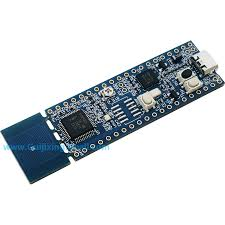
\includegraphics[width=0.3\textwidth]{Imagenes/LPC845.png}
    \end{center}
    \begin{itemize}
        \item \textbf{Microcontrolador:} LPC845 de NXP, basado en núcleo ARM Cortex-M0+.
        \item \textbf{Frecuencia de reloj:} Hasta 30 MHz.
        \item \textbf{Memoria Flash:} 64 KB.
        \item \textbf{Memoria RAM:} 16 KB.
        \item \textbf{Entradas/Salidas:} 34 pines GPIO.
        \item \textbf{Comunicación:} SPI, I2C, UART.
        \item \textbf{Alimentación:} 3.3V a 5V (puede ser alimentado por USB).
        \item \textbf{Interfaz:} USB 2.0 (para programación y depuración).
        \item \textbf{Características adicionales:} Soporta programación en JTAG, dispositivo compatible con FreeRTOS.
        \item \textbf{Datasheet:} 
        \href{https://www.nxp.com/products/processors-and-microcontrollers/arm-microcontrollers/general-purpose-mcus/lpc800-arm-cortex-m0-plus-/lpc845-breakout-board-for-lpc84x-family-mcus:LPC845-BRK}{LPC845 Datasheet}
    \end{itemize}

    \item \textbf{AD620 - Amplificador Instrumental} 
    \begin{center}
        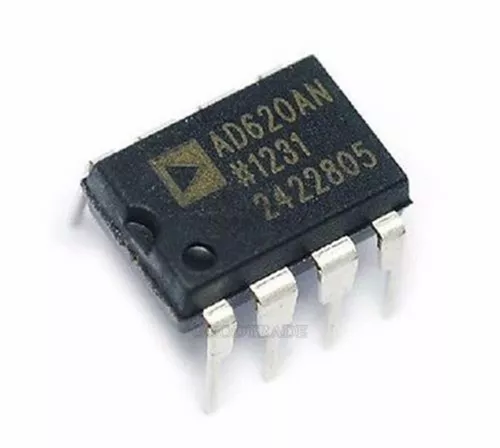
\includegraphics[width=0.3\textwidth]{Imagenes/AD620 component.png}
    \end{center}
    \begin{itemize}
        \item \textbf{Rango de ganancia:} 1 a 1000 (ajustable con una resistencia externa).
        \item \textbf{Precisión:} Baja deriva de offset (50 µV).
        \item \textbf{Alimentación:} ±2.3V a ±18V o 4.6V a 36V (doble y simple).
        \item \textbf{Consumo:} 1.3 mA típico.
        \item \textbf{Ancho de banda:} 120 kHz para ganancia de 100.
        \item \textbf{Datasheet:} \href{https://www.analog.com/media/en/technical-documentation/data-sheets/AD620.pdf}{AD620 Datasheet}
    \end{itemize}

    \item \textbf{MAX6675 - Convertidor Termocupla a Digital} 
    \begin{center}
        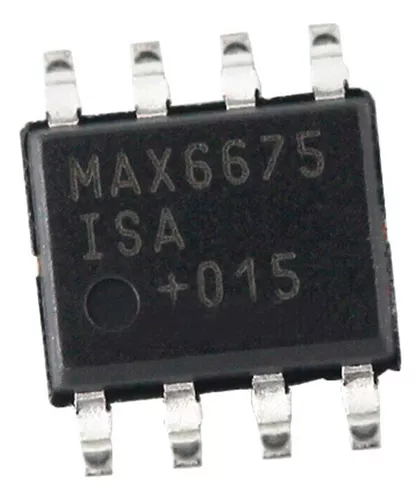
\includegraphics[width=0.3\textwidth]{Imagenes/max6675 component.png}
    \end{center}
    \begin{itemize}
        \item \textbf{Tipo de termocupla:} Compatible con termocupla tipo K.
        \item \textbf{Resolución:} 12 bits (0.25°C por LSB).
        \item \textbf{Rango de medición:} 0°C a +1024°C.
        \item \textbf{Interface:} SPI (4-wire).
        \item \textbf{Alimentación:} 3.0V a 5.5V.
        \item \textbf{Consumo:} 1.5 mA típico.
        \item \textbf{Datasheet:} \href{https://datasheets.maximintegrated.com/en/ds/MAX6675.pdf}{MAX6675 Datasheet}
    \end{itemize}

    \item \textbf{MAX31865 - Convertidor para Termistor RTD (PT100/PT1000)} 
    \begin{center}
        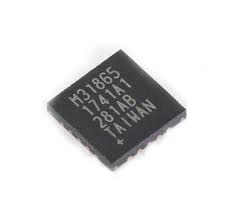
\includegraphics[width=0.3\textwidth]{Imagenes/MAX31685 component.jpg}
    \end{center}
    \begin{itemize}
        \item \textbf{Tipo de sensor:} PT100 o PT1000.
        \item \textbf{Resolución:} 15 bits.
        \item \textbf{Rango de temperatura:} -200°C a +850°C.
        \item \textbf{Interface:} SPI.
        \item \textbf{Alimentación:} 3.0V a 5.5V.
        \item \textbf{Consumo:} 5 mA típico (activo), 0.3 µA (en reposo).
        \item \textbf{Datasheet:} \href{https://datasheets.maximintegrated.com/en/ds/MAX31865.pdf}{MAX31865 Datasheet}
    \end{itemize}

    \item \textbf{LM311 - Comparador de Voltaje} 
    \begin{center}
        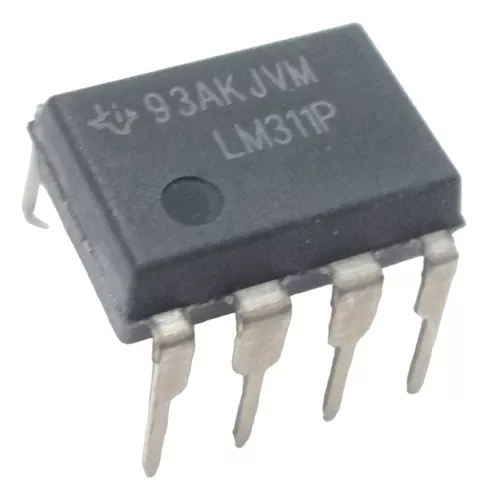
\includegraphics[width=0.3\textwidth]{Imagenes/LM311 Component.png}
    \end{center}
    \begin{itemize}
        \item \textbf{Tiempo de respuesta:} 200 ns (típico).
        \item \textbf{Alimentación:} 3V a 32V (simple), ±1.5V a ±16V (doble).
        \item \textbf{Corriente de entrada:} 300 nA (máx).
        \item \textbf{Salida:} Colector abierto (requiere resistencia de pull-up).
        \item \textbf{Rango de temperatura de operación:} -40°C a +85°C.
        \item \textbf{Datasheet:} \href{https://www.ti.com/lit/ds/symlink/lm311.pdf}{LM311 Datasheet}
    \end{itemize}

    \item \textbf{4N25 - Optoacoplador} 
    \begin{center}
        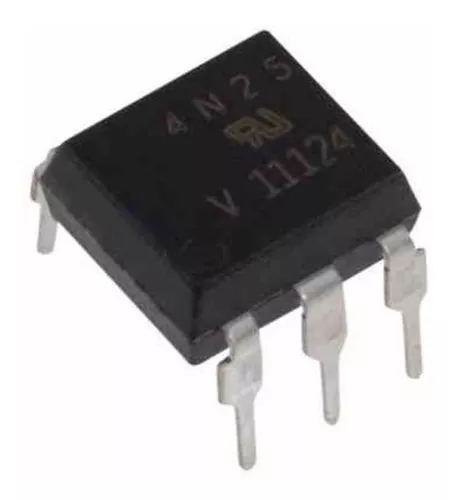
\includegraphics[width=0.3\textwidth]{Imagenes/4N25 component.png}
    \end{center}
    \begin{itemize}
        \item \textbf{Aislamiento:} 5000 VRMS.
        \item \textbf{Tensión de entrada (LED):} Máx 1.2V a 20 mA.
        \item \textbf{Corriente de colector:} 50 mA (máx).
        \item \textbf{Tiempo de respuesta:} 2 µs (típico).
        \item \textbf{Alimentación del transistor:} Hasta 30V.
        \item \textbf{Datasheet:} \href{https://www.vishay.com/docs/83725/4n25.pdf}{4N25 Datasheet}
    \end{itemize}

    \item \textbf{LM358 - Amplificador Operacional Dual} 
    \begin{center}
        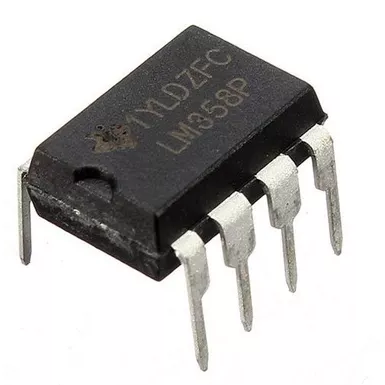
\includegraphics[width=0.3\textwidth]{Imagenes/LM358.png}
    \end{center}
    \begin{itemize}
        \item \textbf{Alimentación:} 3V a 32V (simple), ±1.5V a ±16V (doble).
        \item \textbf{Corriente de consumo:} 0.7 mA por amplificador.
        \item \textbf{Ganancia de voltaje:} 100 dB (típico).
        \item \textbf{Ancho de banda:} 1 MHz (típico).
        \item \textbf{Salida:} Capaz de operar hasta el nivel de tierra (ground).
        \item \textbf{Datasheet:} \href{https://www.ti.com/lit/ds/symlink/lm358.pdf}{LM358 Datasheet}
    \end{itemize}

    \item \textbf{Relés - Songle SRD-05VDC-SL-C} 
    \begin{center}
        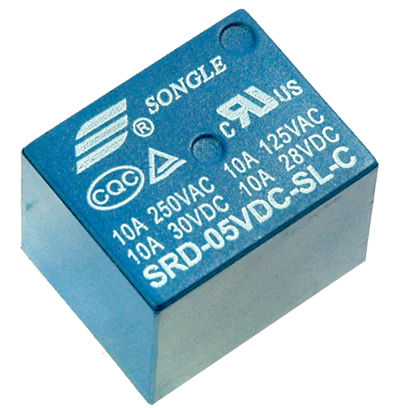
\includegraphics[width=0.3\textwidth]{Imagenes/rele component.png}
    \end{center}
    \begin{itemize}
        \item \textbf{Modelo:} Songle SRD-05VDC-SL-C.
        \item \textbf{Tensión de bobina:} 5V DC (controlados por los pines de la placa).
        \item \textbf{Capacidad de corriente:} Hasta 10A a 250V AC o 10A a 30V DC.
        \item \textbf{Configuración de contactos:} SPDT (Single Pole Double Throw).
        \item \textbf{Consumo:} Aproximadamente 70-80 mA por relé cuando está activado.
        \item \textbf{Datasheet:} \href{}{Songle SRD-05VDC-SL-C Datasheet}
    \end{itemize}
\end{itemize}
